%!TEX program = pdflatex

\documentclass[a4paper]{article}
\usepackage{amsmath}
\usepackage{graphicx}
\usepackage{hyperref}
\usepackage{float}
\usepackage{caption}
\usepackage{subcaption}
\usepackage{booktabs}

\title{New York City (NYC) taxi data analysis}
\setcounter{secnumdepth}{-1}
\begin{document}
\newcommand{\plotpath}{plots/}
\maketitle
\section{Introduction}

The yellow taxi is a symbol of New York. It facilities people's daily life by providing convenient transportation service. On average the yellow taxis in the NYC provide 485,000 trips a day. So I may be able to find some of people's interesting behaviors or living patterns by digging into their transportation data, that is, the travel data of those yellow cabs running on the roads of NYC, day and night. 

In specific, I are to identify the answers for the following questions:
\begin{itemize}
\item[-] Understanding taxis distribution. Before answering this question, one may guess that Manhattan has the most taxis among the five districts. But I still don't have a clear idea on the difference between those numbers. How many times of taxis are there in Manhattan compared with Brooklyn? To answer these related questions, I need to figure out the actual distribution of taxis.
\item[-] Identifying the performance of two vehicle-mounted systems. There are two types of those systems, Verifone Transportation Systems (VTS) and Mobile Knowledge Systems Inc (CMT) with the same functionality. Normally there is only one in a taxi. The systems is to help collect trip data, issue payments and so on. It is of interest to identify the market share of these two systems and find out whether passengers will take use of the system to pay taxi fees.
\item[-] Understanding passengers' payment patterns. Among them, one of the most interesting things is about tips. To understand passengers' paying behaviors related to tips, I are here to find answers to the following three questions:
  \begin{itemize}
  \item[1] Tips vs. payment types. Will passengers more willing to use cash to pay tips or credit cards? Considering that the paying taxi fees using credit cards is enabled by the vehicle-mounted systems mentioned above, if I find that passengers are more likely to use cash to pay tips, I can conclude that passengers don't actually use the systems quite Ill.
  \item[1] Tips vs. total fares. By common sense the further a passenger goes, the higher possibility he will pay a high tip. I are here to validate that and also find out whether there are extra findings.
  \item[1] Tips vs. places to go. Will people who go to a hotel pay a higher tip than ones go to a restaurant? In this report I only discuss the following types of places: restaurants, hotels and cinemas.
  \end{itemize}
\end{itemize}
Following is a brief framework of this project.

\section{Exploratory analysis}
\begin{figure}[H]
\begin{center}
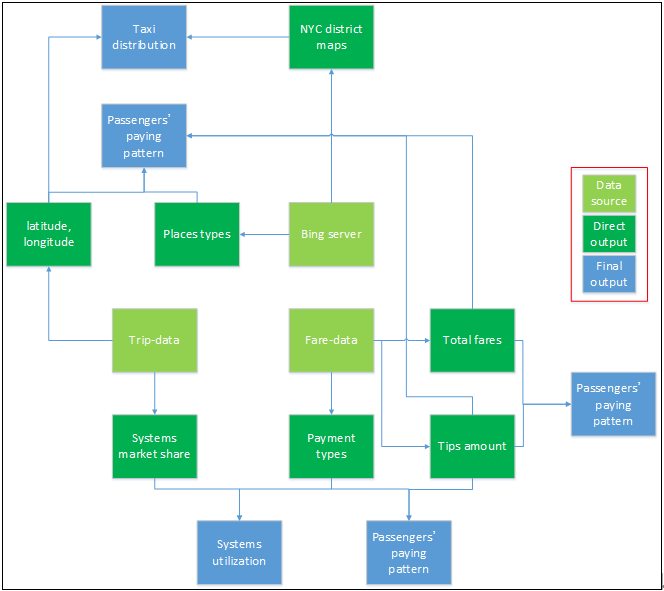
\includegraphics[width=\textwidth]{\plotpath/roadmap.png}
\end{center}
\label{}
\caption{Project framework}
\end{figure}

\section{Dataset}
To answer the above questions, I need to combine multiple data sources:
\begin{itemize}
\item[-] Taxi related data is from \href{http://publish.illinois.edu/dbwork/open-data/}{2013 New York City Taxi Data}. Basically there are two types of csv files in this data set. As mentioned from the linked webpage, ``trip\_fare.csv'' contains data about passengers' payment, and ``trip\_data.csv'' contains data about the trips. Each types of data is in 12 chunks, a chunk per month. In this project, due to the limited time, I only process the data in January. Of those data, what will be used in this project are:
\item[-] \href{https://msdn.microsoft.com/en-us/library/hh478192.aspx}{Bing Map NAVTEQNA}: It is the data source I am to use to handle the location data. The data source contains the data of places of interest (POI) such that I am able to identify the place type by inputting the location data. Normally, by getting the EntityTypeID I am able to refer the \href{https://msdn.microsoft.com/en-us/library/hh478191.aspx}{table} to find the type of place. In this project, I only focus on three types of places: restaurants (`5800'), hotels (`7011') and cinemas (`7832').To get access to the data source, I need to go to Bing Query API, which is mentioned below.
\item[-] \href{https://msdn.microsoft.com/en-us/library/gg585126.aspx}{Bing Query API}: It is a way to get access to the data source NAVTEQNA. There are multiple ways to query, but I will use \href{https://msdn.microsoft.com/en-us/library/gg585133.aspx}{Query by Area} in the project. This is because I can retrieve the all three types of places in one query. It can return results of JSON (used in the project) and XML formats, which is well documented in the linked page. The fundamental variable for the query is the location of the place in the following data structure: (latitude, longitude, distance).
\item[-] \href{https://msdn.microsoft.com/en-us/library/dn306801.aspx}{Bing Geodata API}: To understand the taxis distribution, it is necessary to transform the latitude and the longitude to the district. To achieve that, I use this API in the project, which can return the ``Shape'' of the district that contains the location point. The ``shape'' variable it returns is a string that was previously compressed. By decompressing the string using the decompression algorithm it mentions, I am able to change the string into a list of points that plot the border of the polygon shape. Then what I need to do is to check whether the interested point is in the polygon. The response is either in JSON (used in the project) or XML format, the structure is clearly illustrated in the linked page. 
\end{itemize}

\section{Data processing}
\href{http://publish.illinois.edu/dbwork/open-data/}{2013 New York City Taxi Data} is the major data source I work on in this project. It is the foundation of the data processing later on. The first thing I do is to join two tables by hack license. Then I eliminate the entries with latitude or longitude equal zero, which is the mistakes from GPS when collecting the data. Then I try to get the related district of the location by the following steps:
\begin{itemize}
\item[-] Query the location by inputting (latitude, longitude) from the five districts in NYC through \href{https://msdn.microsoft.com/en-us/library/dn306801.aspx}{Bing Geodata API};
\item[-] Decompress the string I get stored in json['d']['results'][0]['Primitives'][0]['Shape'][2:] of the JSON response, return a list of points that plot the border of the district;
\item[-] Now I have the borders of five districts in NYC. What I need to do now is to check whether the interested point is in the polygon by the \href{http://www.ariel.com.au/a/python-point-int-poly.html}{algorithm}.
\item[-] Considering that there are too many points in a polygon, which will cost much more time when doing the point checking later on. So I use \href{http://postgis.refractions.net/documentation/manual-svn/ST_Simplify.html}{ST\_Simplify} to reduce the number of points.
\end{itemize}

Previously the work flow is designed as query the API each time I have a location point. But it turns out it is extremely time consuming so that I finally decide to check the point locally.

\section{Data visulization}
\subsection{Understanding taxis distribution}
The taxis distribution is demonstrated as below. It can be seen that taxis in Manhattan is extremely high (about 40 times of the second district). Remember that the location I put is where passengers are picked up. This means that people are much more often to take a taxi in Manhattan. If they are at other districts, they may choose other means of transportation. On the other hand, it may be because it is harder to take a taxi in other districts (since all are waiting at Manhattan) so that people can't access to them easily.

\begin{figure}[H]
\begin{center}
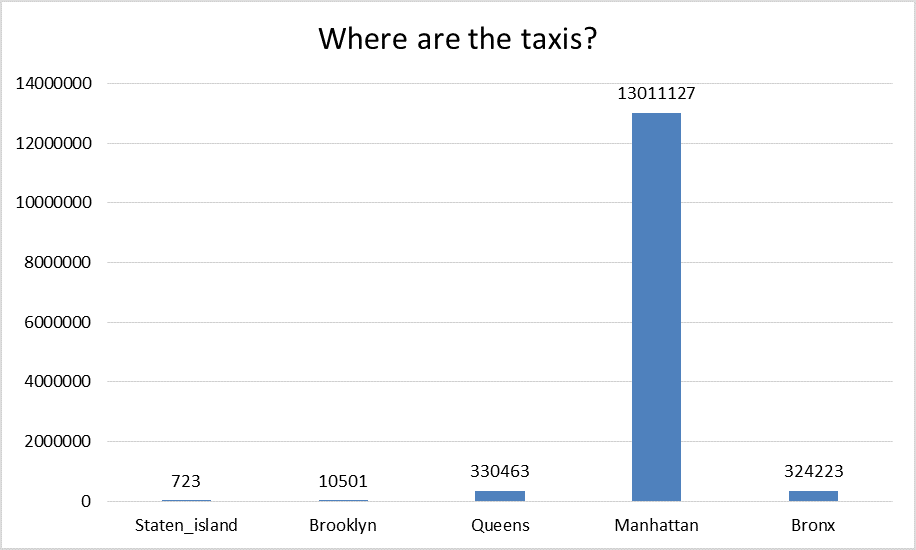
\includegraphics[width=\textwidth]{\plotpath/1.png}
\end{center}
\label{}
\end{figure}

\subsection{Identifying the performance of two vehicle-mounted systems}
It can be seen from the following graph that both systems perform equally. The market share are very close and passengers' paying patterns are almost the same (in terms of using cash or credit cards).

\begin{figure}[H]
\begin{center}
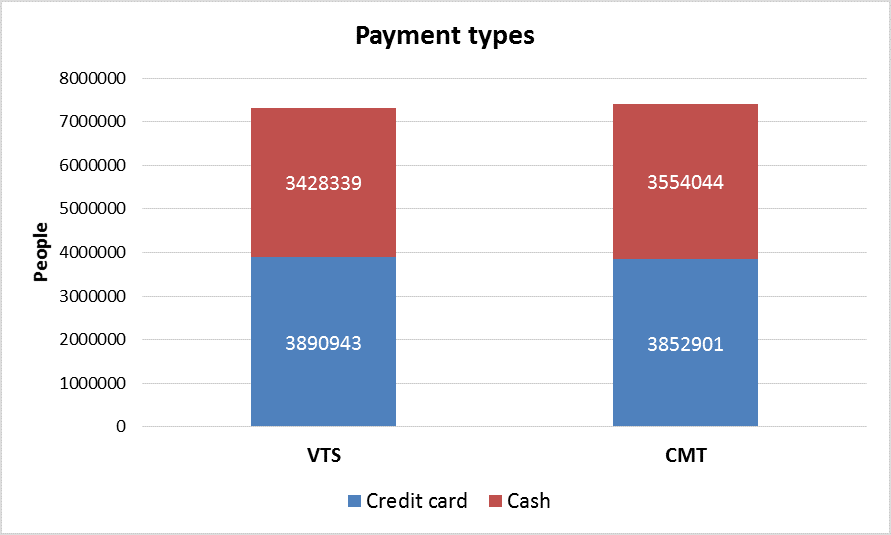
\includegraphics[width=\textwidth]{\plotpath/2.png}
\end{center}
\label{}
\end{figure}

\subsection{Understanding passengers' payment patterns}
It is just the case that passengers will not pay tips using cash (the number is rounded). Interestingly, passengers are ``willing'' to pay two dollars as tips. It seems that people's paying patterns really change due to the usage of the vehicle-mounted systems. But I guess it is partially because in the paying process in those two systems, there is a step asking for tips (it can be skipped) and passengers just want to be nice.

\begin{figure}[H]
\begin{center}
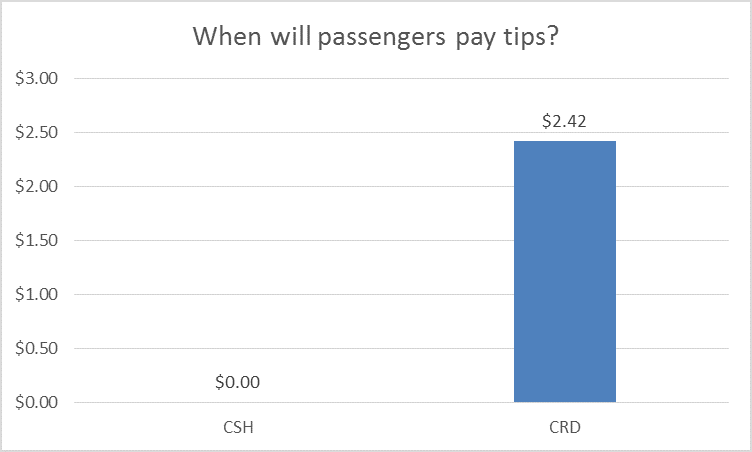
\includegraphics[width=\textwidth]{\plotpath/3.png}
\end{center}
\label{}
\end{figure}

Compared with the base case (`None': \$2.27), I believe there is no difference between the tips paid when going to restaurants or hotels and elsewhere. But maybe people are more willing to pay a higher tips when going to cinemas. This hypothesis should be tested with a larger sample or data sets.

\begin{figure}[H]
\begin{center}
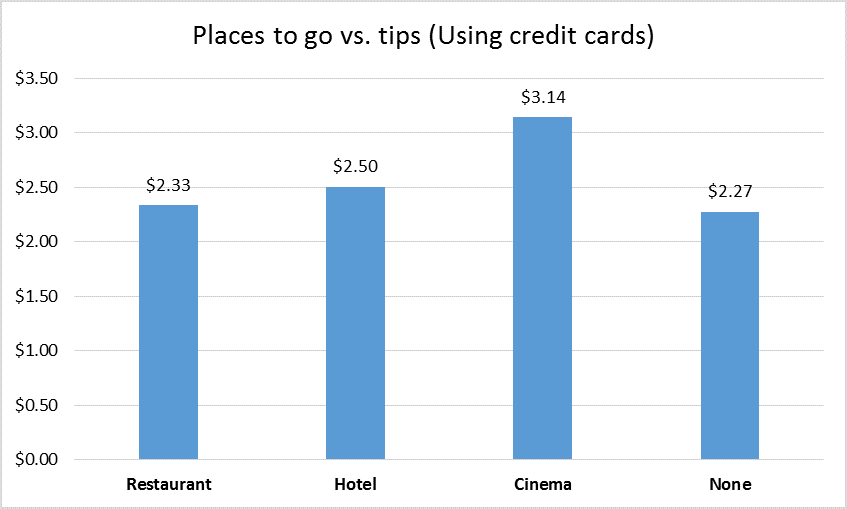
\includegraphics[width=\textwidth]{\plotpath/4.png}
\end{center}
\label{}
\end{figure}

\end{document} 